% Created 2015-01-22 Thu 23:44
\documentclass[11pt]{article}
\usepackage[utf8]{inputenc}
\usepackage[T1]{fontenc}
\usepackage{fixltx2e}
\usepackage{graphicx}
\usepackage{longtable}
\usepackage{float}
\usepackage{wrapfig}
\usepackage{rotating}
\usepackage[normalem]{ulem}
\usepackage{amsmath}
\usepackage{textcomp}
\usepackage{marvosym}
\usepackage{wasysym}
\usepackage{amssymb}
\usepackage{hyperref}
\tolerance=1000
\usepackage{algorithmic}
\usepackage{mathtools}
\author{Xiaolong Zhang}
\date{2015-01-16 Fri}
\title{Stanford Machine Learning Notes}
\hypersetup{
  pdfkeywords={Machine Learning,notes},
  pdfsubject={This is the notes when I'm learning Stanford Machine Learning on Coursera},
  pdfcreator={Emacs 24.3.1 (Org mode 8.2.10)}}
\begin{document}

\maketitle
\section*{Info}
\label{sec-1}
URL is \url{https://class.coursera.org/ml-005/lecture}

\section*{Introduciton}
\label{sec-2}
\subsection*{What is machine learning}
\label{sec-2-1}
\begin{itemize}
\item Arthur Samuel (1959): \textbf{Field of study of that gives computers the ability to learn without being explicitly programmed.}
\item Tom Mitchel (1998): A Well-posed Learning Problem is *A computer program is said to learn from experience E with repsect to some task T and some performance measure P, if its performance on T, as measured by P, improves with experience E.
\end{itemize}
\subsection*{Machine learning algorithms:}
\label{sec-2-2}
We mainly talks about \textbf{two types of algorithm}:
\begin{itemize}
\item Supervised Learning
\item Unsupervised Learning
\item Others: Reinforcement Learning, Recommender System.
\end{itemize}
And \textbf{Practical advice for applying learning algorithm}
\subsubsection*{Supervised Learning}
\label{sec-2-2-1}
"Right Answers" are given. 
\begin{itemize}
\item Regression (Housing price prediction)
\label{sec-2-2-1-1}
Predict continuous valued output (price)
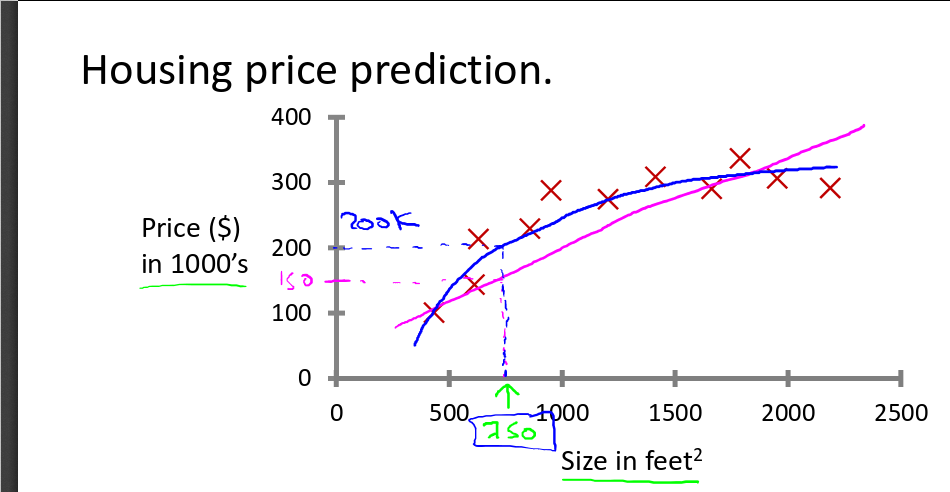
\includegraphics[width=.9\linewidth]{./images/screenshot-01.png}
\item Classification (Breast cancer (malignant, benign)
\label{sec-2-2-1-2}
Discrete valued output (0 or 1)
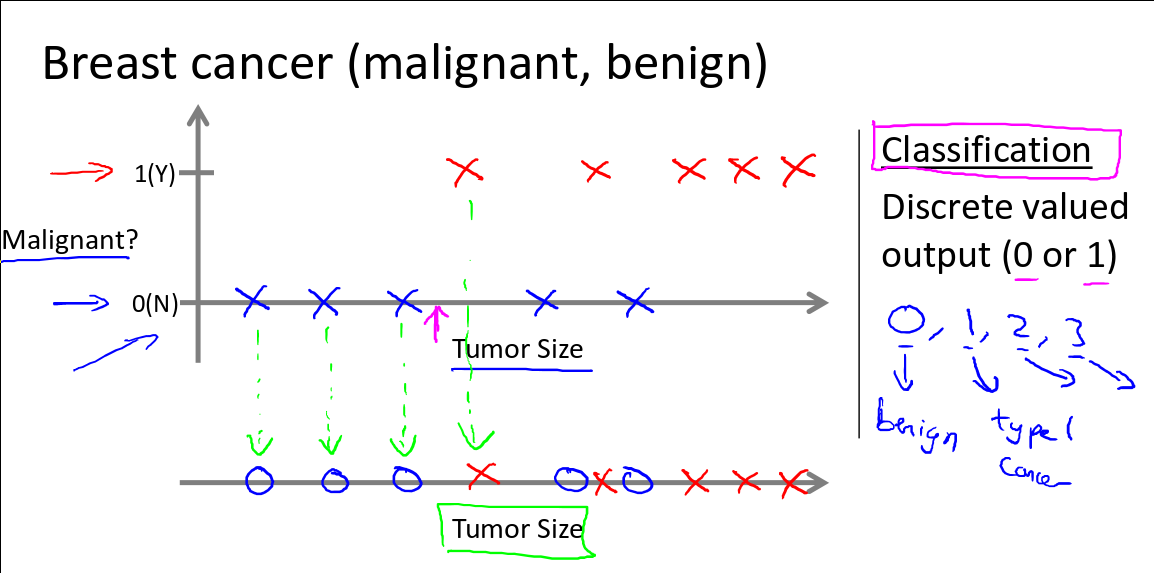
\includegraphics[width=.9\linewidth]{./images/screenshot-02.png}
\end{itemize}

\subsubsection*{Unsupervised Learning}
\label{sec-2-2-2}
No knowledge is given.
\begin{itemize}
\item Google News Grouping
\label{sec-2-2-2-1}
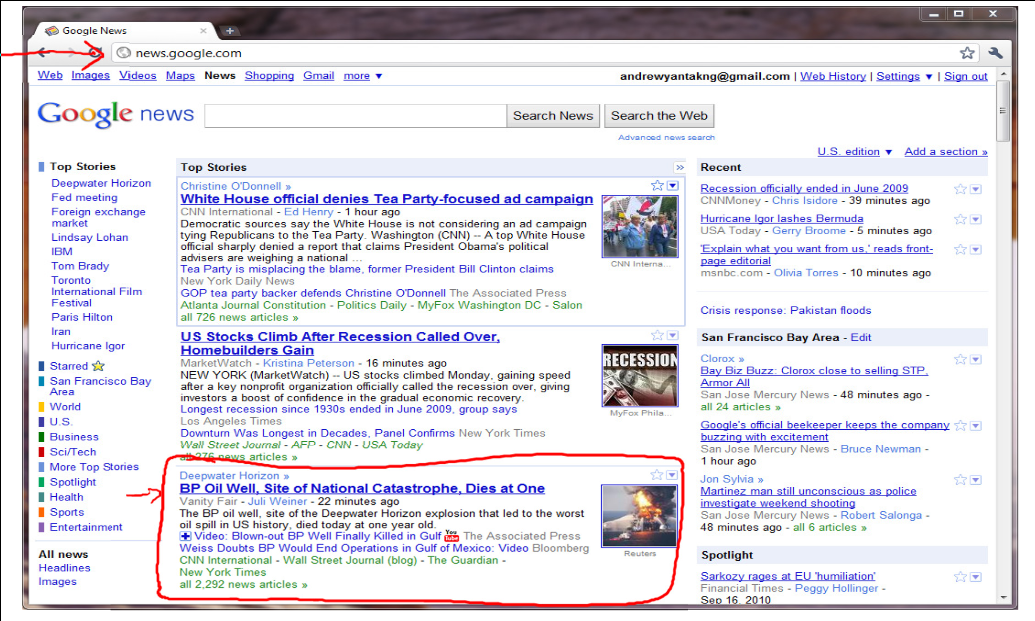
\includegraphics[width=.9\linewidth]{./images/screenshot-03.png}
\item Cocktail party problem
\label{sec-2-2-2-2}
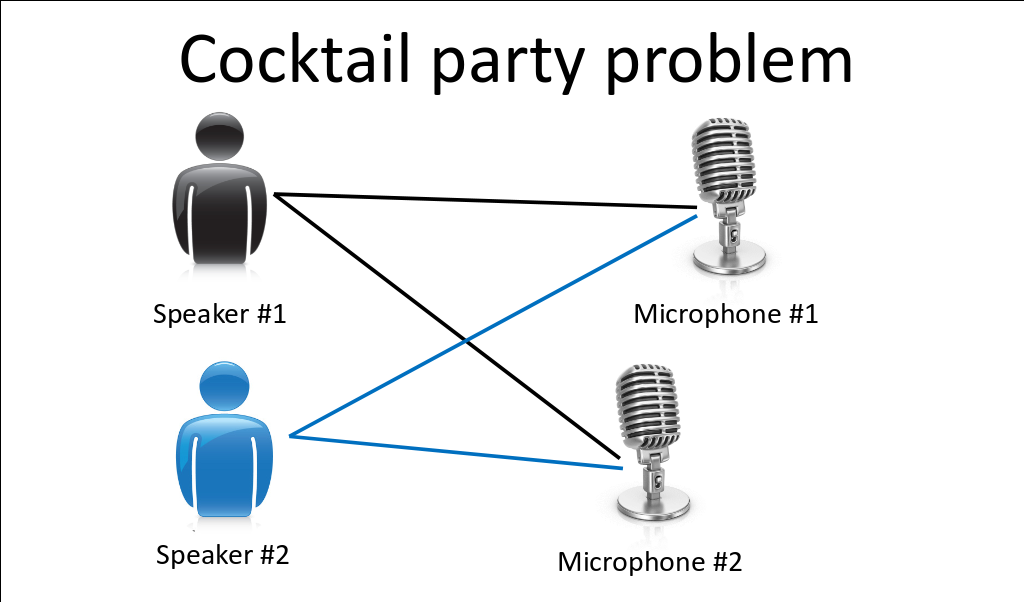
\includegraphics[width=.9\linewidth]{./images/screenshot-04.png}
\end{itemize}
\section*{Linear Regression}
\label{sec-3}
\subsection*{Model Representation}
\label{sec-3-1}
Notations:
\begin{enumerate}
\item \(m\) is Number of training examples.
\item \(x\)'s is "input" variable  / feature.
\item \(y\)'s is "output" variable / "target" variables.
\item \((x,y)\) is one training example.
\item \((x^{(i)},y^{(i)})\) is the \(i\)th example, \(i\) starts from \(0\).
\item \(h\) is called hypothesis, it maps the input to output. In this lecture, we represent \(h\) using linear function, thus it's called \textbf{linear regression}. For linear regression with one variable, it's called \textbf{univariate linear regression}. For example, the \textbf{univariate linear regression} is usually written as: \(h_\theta (x) = \theta_0 + \theta_1 x\). The \(\theta\) here represents the coefficient variables. Sometimes it's written as \(h(x)\) as a shorthand.
\end{enumerate}
\subsection*{Cost Function}
\label{sec-3-2}
Since the hypothesis is written as \(h_\theta (x) = \theta_0 + \theta_1 x\), where \(\theta_i\)'s are the parameters, then how to choose \(\theta_i\)'s?
The idea is to choose \(\theta_0, \theta_1\) so that \(h_\theta (x)\) is close to \(y\) for our training examples \((x,y)\). More formally, we want to
\[
\underset{\theta_0,\theta_1}{\text{minimize}} \frac{1}{2m}\sum_{i=1}^{m}\left( h_\theta(x^{(i)}) - y^{(i)} \right)^2
\],
where \(m\) is the number of trainnig examples. To recap, we're minimizing half of the averaging error. Note that the variable here are \(\theta\)s, and \(x\) and \(y\)'s are constants.

By convention, we define the \textbf{cost function} \(J(\theta_0,\theta_1)\) to represent the objective function. That is
\begin{gather*}
J(\theta_0,\theta_1) = \frac{1}{2m}\sum_{i=1}^{m}\left( h_\theta(x^{(i)}) - y^{(i)} \right)^2 \\
\underset{\theta_0,\theta_1}{\text{minimize}} J(\theta_0,\theta_1)
\end{gather*}

This cost function is also called \textbf{squared error function}. There are other cost functions, but it turns out that squared error function is a resonable choice and will work for most of regression problem.
\subsection*{Cost Function Intuition}
\label{sec-3-3}
Before getting a intuition about the cost function, let's have a recap, we now have
\begin{enumerate}
\item Hypothesis: \[h_\theta (x) = \theta_0 + \theta_1 x\]
\item Parameters: \[\theta_0,\theta_1\]
\item Cost Function: \[J(\theta_0,\theta_1) = \frac{1}{2m}\sum_{i=1}^{m}\left( h_\theta(x^{(i)}) - y^{(i)} \right)^2 \]
\item Goal: \[\underset{\theta_0,\theta_1}{\text{minimize}} J(\theta_0,\theta_1)\]
\end{enumerate}

In order to visualize our cost function, we use a simplified hypothesis function: \(h_\theta (x) = \theta_1 x\), which sets \(\theta_0\) to \(0\). So now we have
\begin{enumerate}
\item Hypothesis: \[h_\theta (x) =  \theta_1 x\]
\item Parameters: \[\theta_1\]
\item Cost Function: \[J(\theta_1) = \frac{1}{2m}\sum_{i=1}^{m}\left( h_\theta(x^{(i)}) - y^{(i)} \right)^2 \]
\item Goal: \[\underset{\theta_1}{\text{minimize}} J(\theta_1)\]
\end{enumerate}

So now let's compare function \(h_\theta (x)\) and function \(J(\theta_1)\):
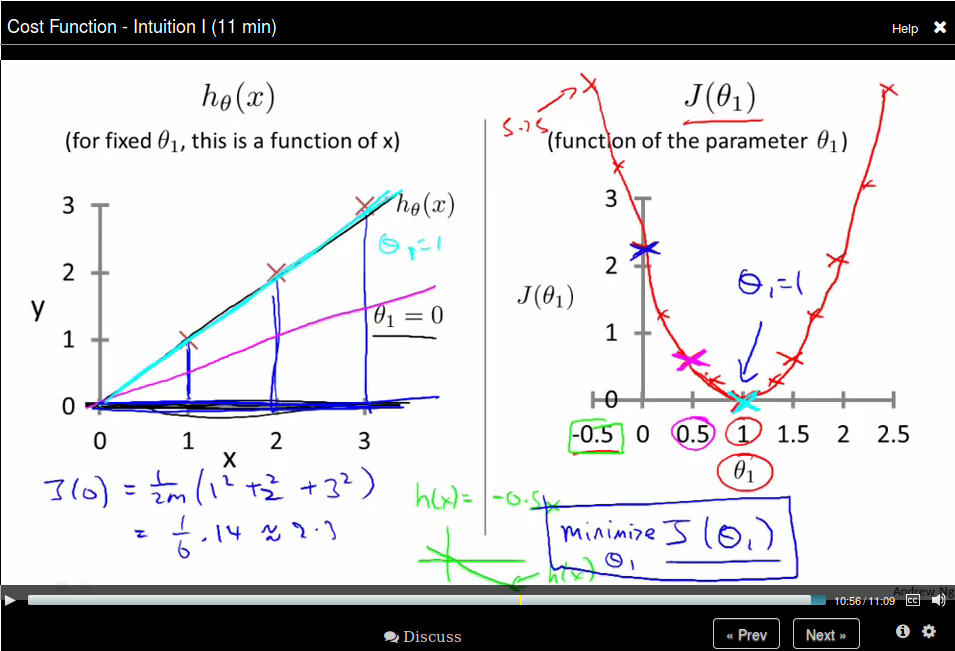
\includegraphics[width=.9\linewidth]{./images/screenshot-05.png}

Then let's come back to the original function, where we don't have the constrain that \(\theta_0 = 0\). The comparison is like
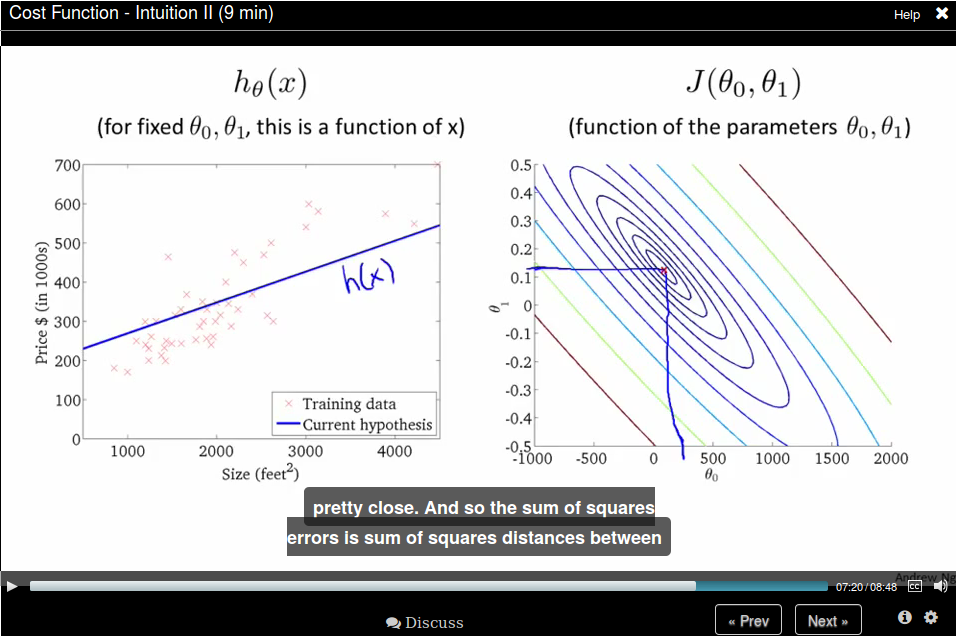
\includegraphics[width=.9\linewidth]{./images/screenshot-06.png}
\subsection*{Gradient Descent}
\label{sec-3-4}
Now we have some function \(J(\theta_0,\theta_1)\) and we want to \(\underset{\theta_0,\theta_1}{\text{minimize}}J(\theta_0,\theta_1)\), we use \textbf{gradient descent} here, which
\begin{enumerate}
\item Start with some \(\theta_0,\theta_1\),
\item Keep changing \(\theta_0,\theta_1\) to reduce \(J(\theta_0,\theta_1)\), until we hopefully end up at a minimum.
\end{enumerate}

To help understand gradient descent, suppose you are standing at one point on the hill, and you want to take a small step to step downhill as quickly as possible, then you would choose the deepest direction to downhill.
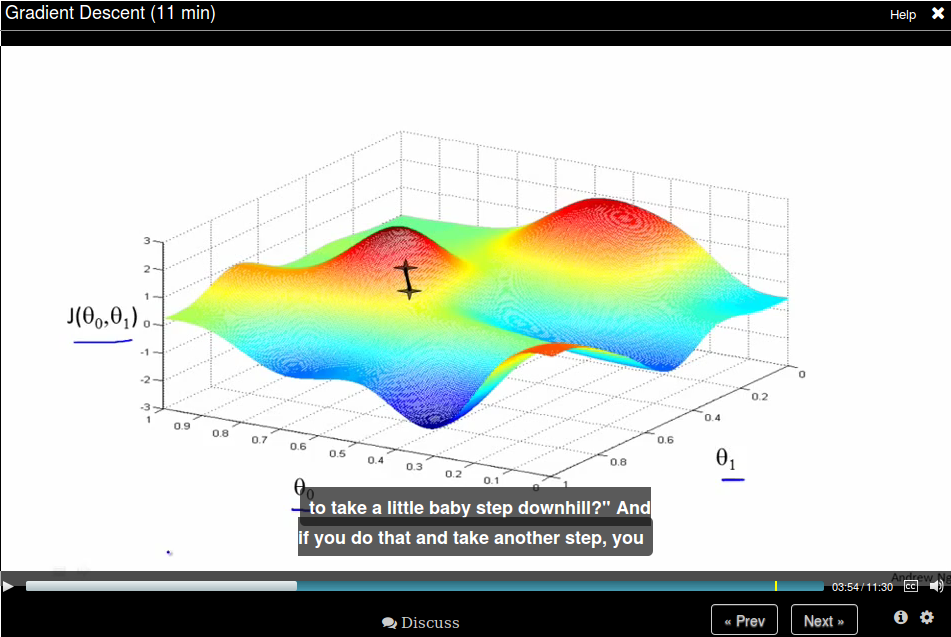
\includegraphics[width=.9\linewidth]{./images/screenshot-07.png}
You keep doing this until to get to a local minimum.
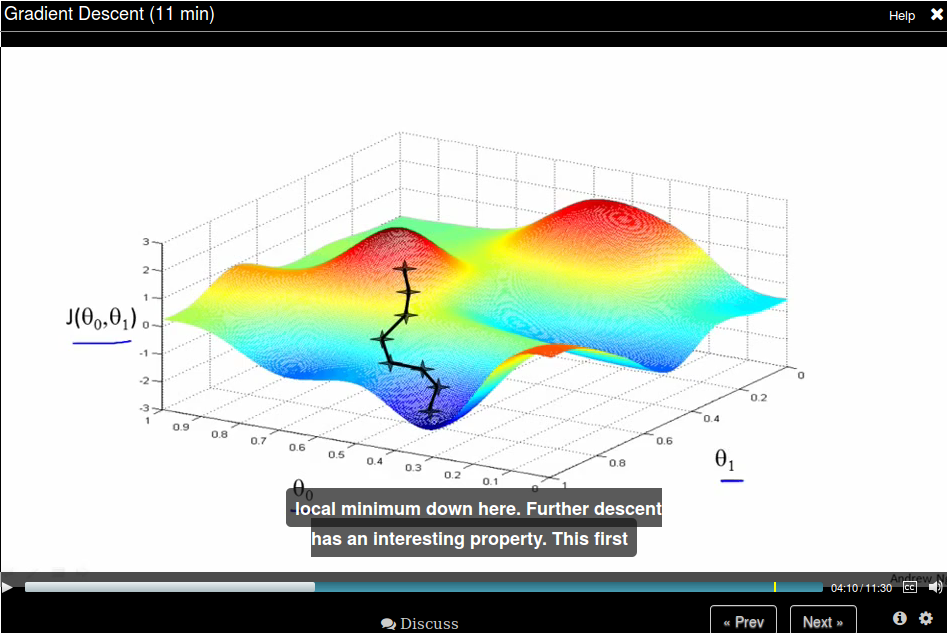
\includegraphics[width=.9\linewidth]{./images/screenshot-08.png}

But if you start with a different initial position, gradient descent will take you to a (very) different position.
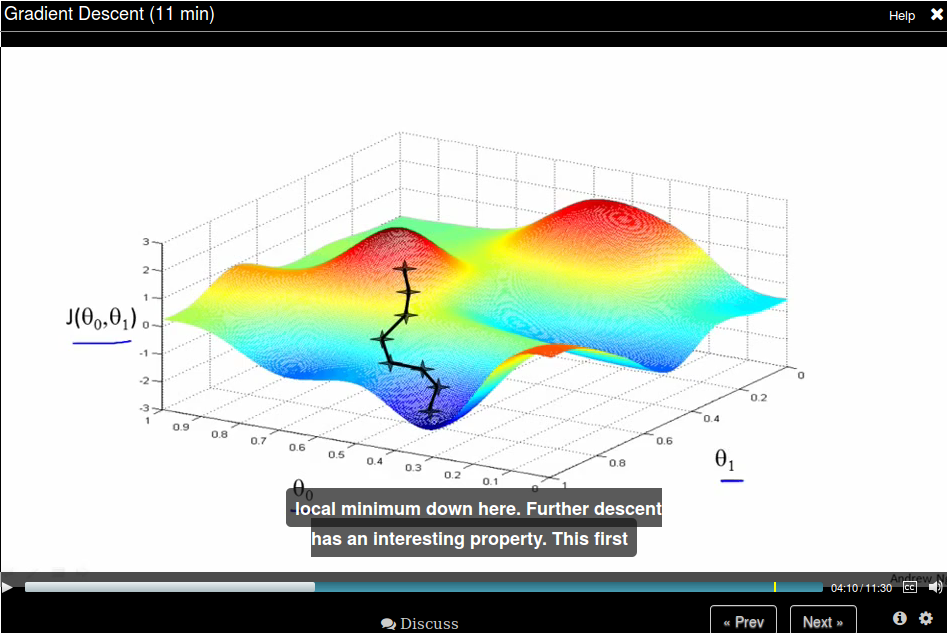
\includegraphics[width=.9\linewidth]{./images/screenshot-08.png}
\subsubsection*{Gradient Descent algorithm}
\label{sec-3-4-1}
We use \(a \coloneqq b\) to represent \textbf{assignment} and \( a = b\) to represent \textbf{truth assertion}.

\begin{algorithmic}
\REPEAT
\STATE $ \theta_j \coloneqq \theta_j - \alpha \frac{\partial}{\partial \theta_j} J(\theta_0,\theta_1) $ \COMMENT{for \(j = 0\) and \(j = 1\)}
\UNTIL{convergence}
\end{algorithmic}

The $\alpha$ here is called learning rate.

Pay attention that when implementing gradient descent, we need to update all $\theta\text{s}$ simultaneous.
% Emacs 24.3.1 (Org mode 8.2.10)
\end{document}